% \documentclass[10pt, hyperref={colorlinks=true,linkcolor=blue},xcolor=dvipsnames]{beamer}
\documentclass{njupre/njupre}

% \usepackage{inconsolata}
% \usepackage[default]{lato}

\title[基于可微渲染的新视角生成方法]{基于可微渲染的新视角生成方法}

\subtitle{ 开题报告 }

\author[朱子航]{\texorpdfstring{
    朱子航 \\ \smallskip 
    \textit{522022150087@smail.nju.edu.cn} \\ \smallskip
    导师:}{}
}

\date[\today]{\texorpdfstring{\today}{}}
\begin{document}
\begin{frame}
    \titlepage
\end{frame}
\begin{frame}
    \frametitle{目录}
    \tableofcontents
\end{frame}

\section{背景介绍}

\subsection{个人简介}

\begin{frame}
    \frametitle{研究生课程修读情况}
        \begin{tabular}{|c|c|c|c|c|}
            \hline
            课程 & 课程编码 & 学分 & 状态 \\
            \hline
            新时代中国特色社会…… & 10284A031 & 2 & 88 \\
            \hline 
            研究生学术规范…… & 10284A030 & 0 & 通过 \\
            \hline
            研究生英语 & 10284A001 & 4 & 免修 \\
            \hline 
            工程伦理 & 10284A006 & 2 & 95 \\
            \hline 
            自然辩证法概论 & 10284A004 & 1 & 86 \\
            \hline 
            线性系统理论 & 0811B0300 & 3 & 76 \\
            \hline
            工程矩阵论 & 085210B01 & 2 & 77 \\
            \hline 
            学术讲座 & 0811D0600 & 1 & 通过 \\
            \hline 
            先进控制技术与应用 & 085210D03 & 3 & 82 \\
            \hline
        \end{tabular}
\end{frame}

\begin{frame}
    $A(2+0+4+2+1)+B(2+3)+C(3+3+2+2+4)+D(1+3)=A(9)+B(5)+C(14)+D(4)=32学分$
    剩余4学分D类课程未修,预计在2024年春夏修读完毕
    \begin{tabular}{|c|c|c|c|c|}
        \hline
        课程 & 课程编码 & 学分 & 状态 \\
        \hline 
        人工智能 & 0811C0500 & 3 & 95 \\
        \hline
        机器学习 & 0811C0700 & 2 & 97 \\
        \hline 
        最优控制理论 & 0811C0400 & 2 & 83 \\
        \hline 
        深度强化学习 & 0811C0600 & 3 & 90 \\
        \hline 
        专业实习 & 0811C1000 & 4 & 完成未计入 \\
        \hline
        群智能系统协作理论与方法 & 0811D1100 & 2 & ing \\
        \hline 
        企业资源管理与控制一体化 & 0811D0200 & 2 & ing \\
        \hline
    \end{tabular}
\end{frame}
\begin{frame}
    \frametitle{AIGC in D5}
    \begin{columns}[c]
        \begin{column}{0.5\textwidth} % Left column width
            \begin{figure}
                \includegraphics[width=0.9\linewidth]{fig_d5_hi.png}
                \caption[short]{AIGC服务\textit{http://www.d5next.ai/}}
            \end{figure}
        \end{column}
        \begin{column}{0.5\textwidth} % Right column width
            \begin{figure}
                \includegraphics[width=0.9\linewidth]{fig_d6_render.png}
                \caption[short]{自研引擎}
            \end{figure}
        \end{column}
    \end{columns}    
\end{frame}
    
\begin{frame}
    \frametitle{CSIG2023流体模拟赛道亚军项目:SPHere}
    \begin{figure}
        \begin{subfigure}{0.74\linewidth}
            \includegraphics[width=0.9\linewidth]{fig_csig2023_app_demo.png}
            \caption[short]{Fluid Simulation Framework}
        \end{subfigure}
        \begin{subfigure}{0.24\linewidth}
            \includegraphics[width=0.9\linewidth]{fig_csig2023_award.jpg}
            \caption{The Second Place in Whole Country}
        \end{subfigure}
    \end{figure}
    \begin{quote}
        使用LuisaCompute \cite{zhengLuisaRenderHighPerformanceRendering2022} 开发了一个高性能的并行流体模拟框架,
        实现了SPH\cite{koschierSmoothedParticleHydrodynamics2020}流体模拟方法
        和加速方法\cite{huangGeneralNovelParallel2019} 最终获得了CSIG2023全国比赛物理模拟分赛道亚军。
    \end{quote}    
\end{frame}

\subsection{课题背景}
\begin{frame}
    \frametitle{学科背景}
    \begin{figure}[H]
        \centering
        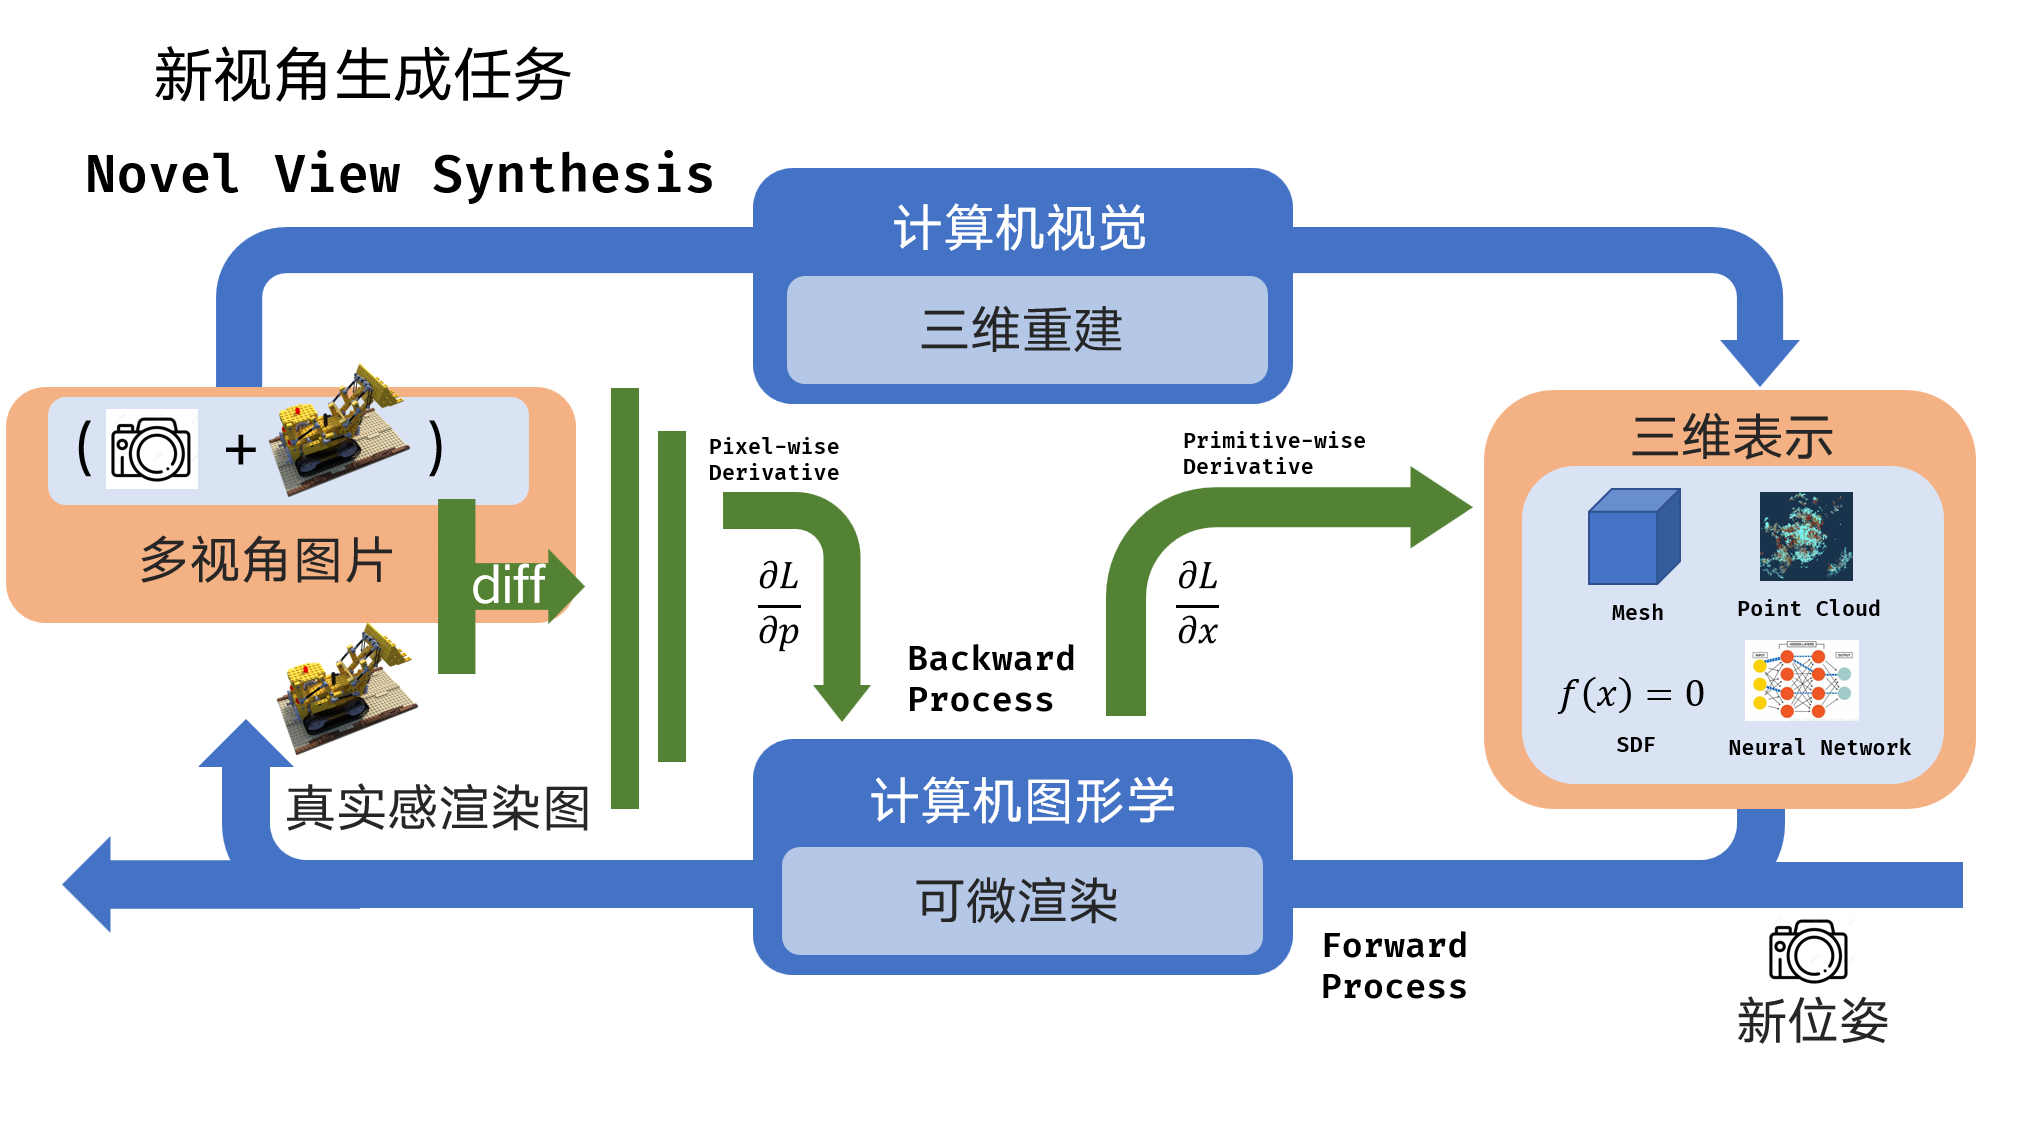
\includegraphics[width=1\linewidth,keepaspectratio]{fig_research_overview.png}
        \caption{学科背景和概述}
        \label{fig:research_overview}
    \end{figure}
\end{frame}

\begin{frame}
    \frametitle{计算机图形学}
    \begin{quote}
        传统意义上,计算机图形学是一门研究如何利用的三维表示和相机模型,
        模拟预测出真实感2D图形并绘制在屏幕上的学科
    \end{quote}
    \begin{figure}[H]
        \centering
        \includegraphics[width=1\linewidth,keepaspectratio]{fig_overview_graphics.png}
        \caption{计算机图形学}
        \label{fig:graphics_overview}
    \end{figure}
\end{frame}

\begin{frame}
    \frametitle{计算机图形学的应用}
    \begin{figure}[ht!]
        \centering
        \begin{subfigure}{0.3\textwidth}
            \centering
            \includegraphics[width=\textwidth]{fig_app_animations_graphics.png}
            \caption{动画}
        \end{subfigure}
        \begin{subfigure}{0.3\textwidth}
            \includegraphics[width=\textwidth]{fig_app_design_graphics.png}
            \caption{设计}
        \end{subfigure}
        \begin{subfigure}{0.3\textwidth}
            \centering
            \includegraphics[width=\textwidth]{fig_app_movie_graphics.png}
            \caption{电影}
        \end{subfigure}
        \begin{subfigure}{0.3\textwidth}
            \includegraphics[width=\textwidth]{fig_app_game_graphics.png}
            \caption{游戏}
        \end{subfigure}
        \begin{subfigure}{0.3\textwidth}
            \centering
            \includegraphics[width=\textwidth]{fig_app_gui_graphics.png}
            \caption{交互界面}
        \end{subfigure}
        \begin{subfigure}{0.3\textwidth}
            \includegraphics[width=\textwidth]{fig_app_visualization_graphics.png}
            \caption{可视化}
        \end{subfigure}
        \caption{计算机图形学的应用}
        \label{fig:app_computer_graphics}
    \end{figure}
\end{frame}

\begin{frame}
    \frametitle{光栅化}
    \begin{figure}[H]
        \centering
        \begin{subfigure}{0.68\textwidth}
            \centering
            \includegraphics[width=\textwidth]{fig_raster_projection.png}
            \caption{光栅化投影:\\ 按物体并行}
        \end{subfigure}
        \begin{subfigure}{0.3\textwidth}
            \includegraphics[width=\textwidth]{fig_raster_sample.png}
            \caption{光栅化采样:\\ 按像素并行}
        \end{subfigure}
    \end{figure}
\end{frame}

\begin{frame}
    \frametitle{光线追踪}
    \begin{figure}[ht!]
        \centering
        \begin{subfigure}{0.48\textwidth}
            \centering
            \includegraphics[width=\textwidth]{fig_ray_tracing_render.png}
            \caption{光线追踪过程示意}
        \end{subfigure}
        \begin{subfigure}{0.48\textwidth}
            \includegraphics[width=\textwidth]{fig_ray_tracing_result_render.png}
            \caption{光线追踪结果}
        \end{subfigure}
    \end{figure}
    \begin{quote}
        按屏幕像素进行并行
    \end{quote}
\end{frame}


\section{研究内容}
\subsection{神经辐射场 Neural Radiance Field (NeRF)}
\begin{frame}
    \frametitle{体渲染器}
    \begin{figure}
        \centering
        \includegraphics[width=\linewidth]{fig_volume_rendering.png}
        \caption[short]{体渲染器原理}
    \end{figure}
\end{frame}

\begin{frame}
    \frametitle{光线步进算法(Ray March)}
    \begin{itemize}
        \item 对于每一根射线,从初始距离$t_n$开始,到最远距离$t_f$为止,步步采样每个位置的颜色$c(t)$和密度$\sigma(t)$
        \item 最终像素是射线上的样本加权和:$C(\mathbf{r})=\int_{t_n}^{t_f}T(t)\sigma(\mathbf{r}(t))\mathbf{c}(\mathbf{r}(t),\mathbf{d})dt$
        \item 此处$T(t)=exp(-\int_{t_n}^{t}\sigma(\mathbf{r}(s))ds)$代表t之后的颜色依然可以残留多少
    \end{itemize}
    \begin{figure}
        \begin{subfigure}{0.48\textwidth}
            \includegraphics[width=\linewidth]{fig_ray_march.png}
            \caption[short]{光线步进}
        \end{subfigure}
        \begin{subfigure}{0.48\textwidth}
            \includegraphics[width=\linewidth]{fig_ray_march_shade.png}
            \caption[short]{传统光估计}
        \end{subfigure}
    \end{figure}
\end{frame}
\begin{frame}
    \frametitle{用神经网络估计$c(t)$和$\sigma(t)$}
    \begin{figure}[H]
        \centering
        \includegraphics[width=0.9\linewidth,keepaspectratio]{fig_nerf_principle.jpg}
        \caption{神经辐射场原理}
        \label{fig:nerf_principle}
    \end{figure}
    $c(t),\sigma(t)=MLP(\mathbf{x}(t),\mathbf{d}(t))$
    \begin{itemize}
        \item 通过引入MLP,将整个渲染过程变成了一种可微的过程,从而实现了一个可微的体渲染器
        \item 与通常的神经网络不同,此处MLP的角色更类似点云,网格等存储格式
        \item 最终预测效果达到大幅度的提升,在集成数据集800x800的图片上PSNR达到了30+
    \end{itemize}
\end{frame}

\begin{frame}
    \frametitle{新视角生成问题数据集}
    \begin{figure}[H]
        \includegraphics[width=0.9\linewidth]{fig_demo_nerf_dataset.png}
        \caption[short]{渲染得到不同视角图片}
    \end{figure}
\end{frame}

\begin{frame}
    \frametitle{NeRF之后的开放问题}
    \begin{itemize}
        \item 更高的精度
        \item 更快的训练与推理速度
        \item 支持特殊场景(动态,反射,暗光,大场景)
        \item 支持编辑(材质,光照,前后景分割等)与泛化
        \item 拓展任务(与Diffusion, SAM等结合)与应用
    \end{itemize}
\end{frame}

\begin{frame}
    \frametitle{近三年NeRF的发展 -- 更高的精度}
    \begin{itemize}
        \item MipNeRF \cite{barronMipNeRFMultiscaleRepresentation2021} 降低模糊
        \item 2022 CVPR Mip NeRF 360 \cite{barronMipNeRF360Unbounded2022} 降低模糊并支持360度全景
        \item 2023 CVPR Zip NeRF \cite{barronZipNeRFAntiAliasedGridBased2023} 进一步引入了NGP的hash encoding
        \item 2023 CVPR NeRFLix \cite{zhouNeRFLiXHighQualityNeural2023} 高清NeRF
    \end{itemize}
\end{frame}

\begin{frame}
    \frametitle{近三年NeRF的发展 -- 更快的速度}
    \begin{itemize}
        \item 2022 CVPR: PointNeRF\cite{xuPointNeRFPointbasedNeurala} 将NeRF变换为特征点云
        \item 2022 CVPR: Direct Voxel Grid Optimization Super Fast Convergence for Radiance  Fields Reconstruction \cite{sunDirectVoxelGrid2022} 使用体素混合MLP
        \item 2022 CVPR: Plenoxels \cite{yuPlenoxelsRadianceFields2021} 完全使用稀疏体素而放弃MLP进行新视角识别
        \item 2022 SIGGRAPH: Instant NGP \cite{mullerInstantNeuralGraphics2022} 使用多精度空间哈希编码将大网络转化为小网络,从而将速度优化到了实时
        \item 2023 MeRF\cite{reiserMERFMemoryEfficientRadiance2023} 减少内存占用
        \item 2023 SIGGRAPH: 3D Gaussian Splatting \cite{kerbl3DGaussianSplatting2023} 使用3D高斯,放弃MLP进行机器学习优化,获得了当前SOTA的精度和效率
    \end{itemize}
    \begin{quote}
        绝大部分的加速措施都需要修改原本的网络,将其中神经网络的部分尽可能地减少甚至消除
    \end{quote}
\end{frame}

\begin{frame}
    \frametitle{近三年NeRF的发展 -- 特殊的场景}
    \begin{itemize}
        \item 2021 CVPR NeRF in the wild \cite{martin-bruallaNeRFWildNeural2021} 不受限制的室外场景
        \item 2023 CVPR Deblur NeRF \cite{leeDPNeRFDeblurredNeural2023} 去镜头模糊
        \item 2023 CVPR Large Urban Scene \cite{xuGridguidedNeuralRadiance2023} 大规模城市场景(复现困难?)
        \item 2022 CVPR D-NeRF \cite{pumarolaDNeRFNeuralRadiance2021} 基于基准场景和变换的动态场景
        \item 2023 CVPR k-planes \cite{KPlanesExplicitRadiance2023} 使用正交投影来支持4D动态场景
    \end{itemize}
\end{frame}

\begin{frame}
    \frametitle{近三年NeRF的发展 -- 编辑与泛化}
    \begin{itemize}
        \item 2023 CVPR Nope NeRF \cite{bianNoPeNeRFOptimisingNeural2023} 不需要相机位姿的NeRF
        \item 四面体网格 tetrahedra\cite{kulhanekTetraNeRFRepresentingNeural2023} 方便后续编辑
    \end{itemize}
\end{frame}

\begin{frame}
    \frametitle{近三年NeRF的发展 -- 拓展与应用}
    \begin{itemize}
        \item 2022 CVPR CLIP NeRF\cite{wangCLIPNeRFTextandImageDriven2022} 尝试了使用文本到场景的转换
        \item 2021 CVPR GIRAFFE \cite{niemeyerGIRAFFERepresentingScenes2021} 使用NeRF作为GAN的后处理生成场景
        \item 2022 CVPR GIRAFFE HD \cite{xueGIRAFFEHDHighResolution2022} 更高清的GIRAFFE
        \item 2023 CVPR Lift3D \cite{liLift3DSynthesize3D2023} 使用3D GAN进行后续生成
        \item Dream Fusion \cite{pooleDreamFusionTextto3DUsing2022} 将 Diffusion Model和NeRF结合,利用SDS loss实现文本控制3D模型生成
    \end{itemize}
\end{frame}
\subsection{高斯溅射 Gaussian Splatting}
\begin{frame}
    \frametitle{另一种渲染器:点云渲染器}
    \begin{figure}[H]
        \centering
        \includegraphics[width=1\linewidth,keepaspectratio]{fig_splatting.png}
        \caption{溅射splatting示意图}
        \label{fig:tile_render}
    \end{figure}
    \begin{quote}
        一个空间中的3D Gaussian经过这个过程会形式化地转变为一个相机平面上的2D Gaussian,可以用相机平面位置 $(x_k,y_k)$和2D协方差矩阵$V_c$表示 
    \end{quote}
\end{frame}

\begin{frame}
    \frametitle{Gaussian Splatting \cite{kerbl3DGaussianSplatting2023}}
    高斯“抛雪球”本质上是构建了一个以3D高斯为基本单元的可微点云渲染器,
    将空间中的光度粒子看做若干3D高斯分布,
    每一个高斯分布都可以用如下参数描述
    \begin{enumerate}
        \item 高斯分布均值位置 $\bf{p}$,是一个空间中的三维坐标
        \item 高斯分布的$3\times 3$协方差矩阵$V$,可以理解为一个旋转变换R和一个拉伸变换S的组合 $V=R^TS^TSR$,
            可以简单理解为把一个标准的球形沿着任意三个正交方向的拉伸变形之后得到的椭球
        \item 服从该高斯分布的特征$\bf{X}$,包括颜色和透明度 
    \end{enumerate}
\end{frame}


\begin{frame}
    \frametitle{相机模型:FlipY}
    \begin{figure}[H]
    \centering
    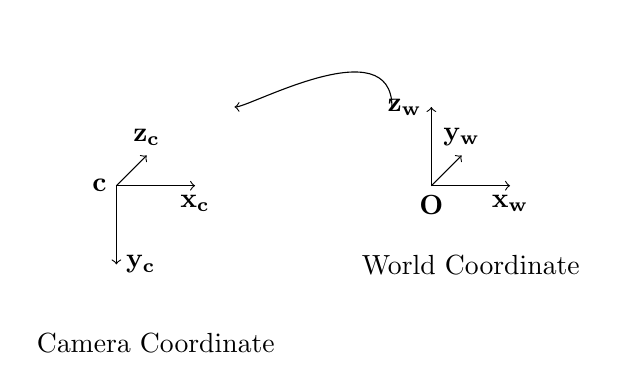
\begin{tikzpicture}[->]
        \begin{scope}[xshift=3.5cm]
            \draw (0,0,0) -- (xyz cs:x=1)node[below]{$\bf{x}_w$};
            \draw (0,0,0) -- (xyz cs:y=1)node[left]{$\bf{z}_w$};
            \draw (0,0,0) -- (xyz cs:z=-1)node[above]{$\bf{y}_w$};
            \node (O) at (0,0,0) [below] {$\bf{O}$};
        \end{scope}
        \draw[->] (3,1) .. controls +(up:1cm) and +(right:0.2cm) .. (1, 1);
        \begin{scope}[xshift=-0.5cm]
            \draw (0,0,0) -- (xyz cs:x=1)node[below]{$\bf{x}_c$};
            \draw (0,0,0) -- (xyz cs:y=-1)node[right]{$\bf{y}_c$};
            \draw (0,0,0) -- (xyz cs:z=-1)node[above]{$\bf{z}_c$};
            \node (P) at (0,0,0) [left] {$\bf{c}$};
        \end{scope}
        \node (A) at (0, -2) {Camera Coordinate};
        \node (B) at (4, -1) {World Coordinate};
    \end{tikzpicture}
    \caption{FlipY Camera Model}
    \label{fig:flip_y_camera}
\end{figure}
\end{frame}

\begin{frame}
    \frametitle{相机模型}
    如图\ref{fig:flip_y_camera}所示,一个正常的右手系世界坐标系$\bf{x_w,y_w,z_w}$和原点$\bf{O}$下,
    相机视角的局部坐标系$\bf{x_c,y_c,z_c}$和相机原点在世界坐标系下的坐标 $\bf{c}$
    $$\left[\begin{matrix} 
        \vec{x}_c \\ \vec{y}_c \\ \vec{z}_c 
    \end{matrix}\right]=
    \left[\begin{matrix} 
        x_{c0} & x_{c1} & x_{c2} \\ 
        y_{c0} & y_{c1} & y_{c2} \\ 
        z_{c0} & z_{c1} & z_{c2} 
    \end{matrix}\right]
    \left[\begin{matrix} 
        \vec{x} \\ \vec{y} \\ \vec{z} 
    \end{matrix}\right]=
    R\left[\begin{matrix} 
        \vec{x} \\ \vec{y} \\ \vec{z} 
    \end{matrix}\right]$$
\end{frame}

\begin{frame}
    \frametitle{视角变换}

    在相机确定之后,任意一个世界坐标$(p_{wx},p_{wy},p_{wz})$都可以经过一个旋转
    和一个平移变换到相机坐标系$(p_{cx},p_{cy},p_{cz})$之中,我们不妨引入齐次坐标的概念
    
    来确定一个$4\times 4$的变换矩阵$\bf{M}$,使得
    
    $[p_{cx},p_{cy},p_{cz},1]=[p_{wx},p_{wy},p_{wz},1]\bf{M}$
    
    并且可以推导出$\bf{M}$的表达式
    
    $$[p_{wx},p_{wy},p_{wz},1]
    \left[\begin{matrix} 
        x_{c0} & y_{c0} & z_{c0} & 0 \\ 
        x_{c1} & y_{c1} & z_{c1} & 0 \\ 
        x_{c2} & y_{c2} & z_{c2} & 0 \\ 
        -\vec{c}\cdot\vec{x}_c &-\vec{c}\cdot\vec{y}_c &-\vec{c}\cdot\vec{z}_c & 1 
    \end{matrix}\right]=[p_{cx},p_{cy},p_{cz}, 1]$$
    
    这里的M被称为View Matrix视角矩阵。
\end{frame}


\begin{frame}
    \frametitle{经过变换的高斯}
    $g_V(x)=\frac{1}{2\pi \sqrt{|V|}}e^{-\frac{1}{2}x^TV^{-1}x}$
    \begin{itemize}
        \item $V$是一个$3\times 3$的协方差矩阵, $|V|$是它的行列式
        \item $x$是一个$3\times 1$的列向量
        \item 高斯变换的好处在于,其傅里叶变换依然是高斯形式:$g_V(x)\leftrightarrow G_V(\omega)=e^{-\frac{1}{2}\omega^TV\omega}=2\pi \sqrt{|V|}g_{V^{-1}}$
    \end{itemize}
    将变换视作重参数化 $y = Mx$
    $g_V(M^{-1}y)=\frac{1}{2\pi\sqrt{|V|}}e^{-\frac{1}{2}(M^{-1}y)^TV^{-1}M^{-1}y}=\frac{|M|}{2\pi\sqrt{|MVM^T|}}e^{-\frac{1}{2}y^T(MVM^T)^{-1}y}=|M|g_{MVM^T}(y)$
    \begin{quote}
    则经过变换得到的y依然服从正态分布,此正态分布是可以定量计算的
    两个高斯分布的卷积也很方便计算: $g_V(x)\otimes g_W(x)=g_{V+W}(x)$
    \end{quote}
\end{frame}

\begin{frame}
    \frametitle{空间往相机平面投影}
    \begin{columns}[c]
        \begin{column}{0.58\textwidth} % Left column width
            \begin{figure}[H]
                \centering
                \includegraphics[width=1\linewidth,keepaspectratio]{fig_surface_splatting.png}
                \caption{可微的高斯变换}
                \label{fig:diff_gaussian_splatting}
            \end{figure}
        \end{column}
        \begin{column}{0.4\textwidth} % Right column width
            $\Phi(t)=[\bold{u}_i,\bold{v}_i,\bold{p}_i]\left[\begin{matrix} \bold{t} \\ 1 \end{matrix}\right]$

            $\bold{x}=m_i(\bold{t})=\left[\begin{matrix} \frac{u_xt_u+v_xt_v+p_x}{u_zt_u+v_zt_v+p_z} \\  \frac{u_yt_u+v_yt_v+p_y}{u_zt_u+v_zt_v+p_z} \end{matrix}\right]$
        \end{column}
    \end{columns}
    \begin{quote}
        从而可以计算Jacobian 
        $$J_i=\left[\begin{matrix}\frac{\partial x}{\partial t_u} & \frac{\partial x}{\partial t_v} \\ \frac{\partial y}{\partial t_u} & \frac{\partial y}{\partial t_v} \end{matrix}\right]=\frac{1}{p_z^2}\left[\begin{matrix}u_xp_z-p_xu_z & v_xp_z - p_xv_z\\ u_yp_z-p_yu_z & v_yp_z-p_yv_z \end{matrix}\right]$$
    \end{quote}
\end{frame}

\begin{frame}
    \frametitle{分块光栅化}
    \begin{figure}[H]
        \centering
        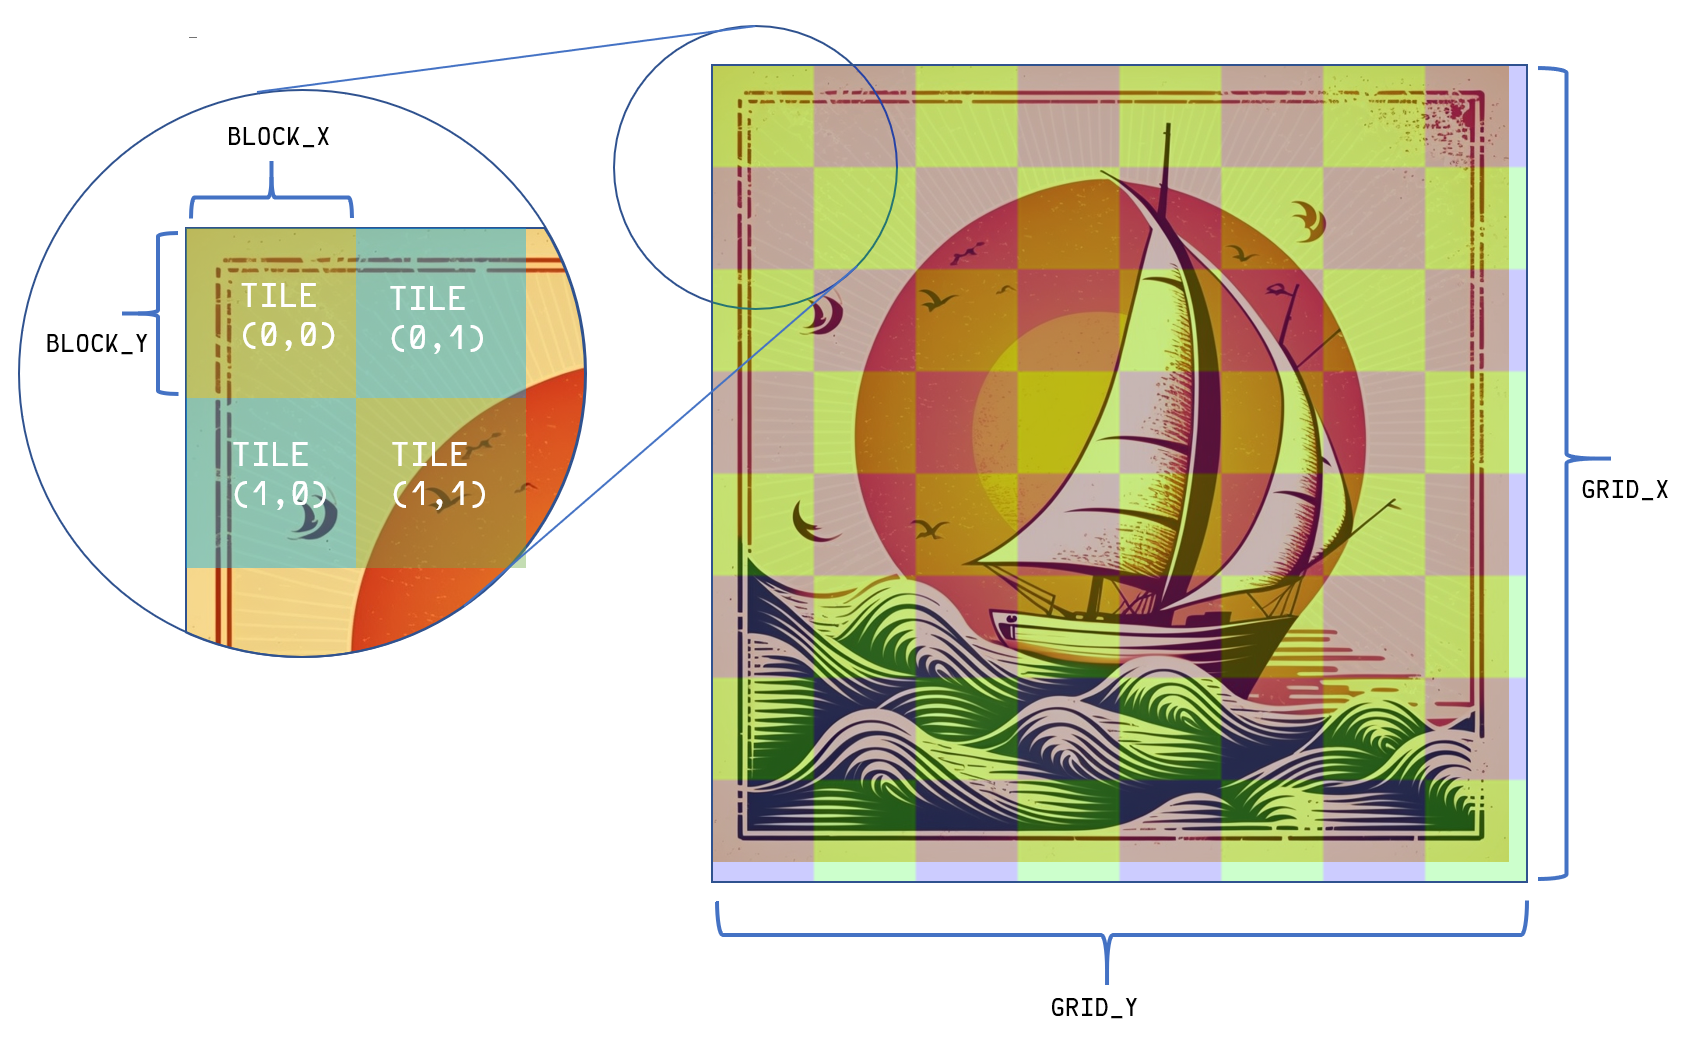
\includegraphics[width=1\linewidth,keepaspectratio]{fig_tile_based_raster.png}
        \caption{分块光栅化}
        \label{fig:tile_render}
    \end{figure}
\end{frame}

\begin{frame}
    \frametitle{分片光栅化}
    \begin{enumerate}
        \item 计算相机的视角变换矩阵和仿射变换矩阵的Jacobian
        \item 将空间转化为为相机局部坐标(变换$\bf{p}$,不变V)
        \item 将相机表面为若干小块(tile),每个小块负责渲染$16\times 16$个像素
        \item 对于每一个tile,可以得到会投影到这个tile上的高斯分布,并将他们按照z轴大小排序
        \item 在NDC中向着相机平面投影,将3D高斯转换为相机平面上的2D高斯分布
        \item 进行band-limit处理来防止aliasing 
        \item 并依排序顺序进行$\alpha$混合,最终得到图像
    \end{enumerate}
\end{frame}

\begin{frame}
    \frametitle{块内$\alpha$混合}
    \begin{quote}
        在经过上述过程之后,每一个块都得到了一个从近到远对应的图像空间Gaussian序列,
        之后我们希望将这个Gaussian列按照一定的透明度顺序进行叠合。需要指出,基于点的高斯
        $\alpha$混合与之前NeRF中的体渲染混合是等价的。
    \end{quote}
    In NeRF
    $C=\sum\limits_{i=1}\limits^{N} T_i(1-exp(-\sigma_i\delta_i))\mathbf{c}_i$, where $T_i=exp(-\sum\limits_{j=1}\limits^{i-1} \sigma_j\delta_j)$
    合并之后,可以把颜色写成每个点颜色的加权和
    $C=\sum\limits_{i}\limits^{N} T_i\alpha_i\mathbf{c}_i$
    此处
    $\alpha_i = (1-exp(-\sigma_i\delta_i))$, $T_i=\prod\limits_{j=1}\limits^{i-1}(1-\alpha_i)$
\end{frame}

\begin{frame}
    \frametitle{后续工作}
    \begin{quote}
        虽然距离Gaussian Splatting源码正式放出不到三个月,arxiv上已经有了一些工作
    \end{quote}
    \begin{itemize}
        \item Dynamic 3D Gaussian \cite{luitenDynamic3DGaussians2023} 来自原作者团队,将Gaussian Splatting 扩展到动态
        \item Dream Gausssian \cite{tangDreamGaussianGenerativeGaussian2023} 将DreamFusion\cite{pooleDreamFusionTextto3DUsing2022}中的NeRF部分替换为3D Gaussian,从而实现了更好的生成质量
    \end{itemize}
\end{frame}

\section{方法介绍}
\begin{frame}
    \begin{quote}
        我在自己的代码框架下复现了Gaussian Splatting的工程,并得到结果如下
    \end{quote}
    \begin{columns}[c]
        \begin{column}{0.48\textwidth}
            \begin{figure}
                \includegraphics[width=\textwidth]{fig_impl_20231018.png}
                \caption{源码结果}
            \end{figure}
        \end{column}
        \begin{column}{0.48\textwidth}
            \begin{figure}
                \includegraphics[width=\textwidth]{fig_reimpl_20231018.png}
                \caption{复现结果}
            \end{figure}
        \end{column}
    \end{columns}
\end{frame}

\begin{frame}
    \frametitle{Gaussian Splatting复现细节}
    \begin{itemize}
        \item pytorch + cuda 混合编程,利用GPU并行计算加速
        \item 使用cuda内部共享内存(shared memory)进行并行算法优化
        \item 使用cub基数排序(radix sort),并行规约(reduce)等算法,
            以及 id chunk等优化方法对于代码效率进行极致的优化
    \end{itemize}
\end{frame}

\begin{frame}
    \frametitle{使用pytorch C++/CUDA扩展}
    使用torch autograd和torch cpp extension 功能可以将一个用C++/CUDA实现的
    高性能并行模块封装为一个torch模块
    \begin{figure}
        \includegraphics[width=0.6\linewidth]{fig_diff_render_20231018.png}
        \caption[short]{可微渲染器优化过程}
    \end{figure}
\end{frame}

\begin{frame}
    \frametitle{idea: 引入全景照片实现前后景分离}
    全景图是一种分辨率为$(2w,w)$的高分辨率图片,其中横轴表示经度$(0,2\pi)$,
    纵轴表示纬度 $(-\frac{\pi}{2},\frac{\pi}{2})$
    \begin{figure}
        \includegraphics[width=0.8\linewidth]{fig_panorama_20231018.png}
        \caption[short]{全景图}
    \end{figure}
\end{frame}

\begin{frame}
    \frametitle{接口: Background}
    \begin{quote}
        在Gaussian Splatting原始的实现中,积累的$T_{final}$最终
        会和背景颜色混合 $C_i=C_{i,gaussian} + T_{final}C_{background}$
        如果我们设计一个可微的全景照片采样器S,
        让每一个像素用相机的姿态都从全景图中进行采样$C_{i,background}=S(i,P_{pano})$
        并将对全景图的微分$T$反向传播到全景图中,就可以优化得到远景。
    \end{quote}
\end{frame}

\begin{frame}
    \frametitle{实现一个可微的全景图片采样器}
    \begin{quote}
        \textbf{双线性插值}
        对于每一个确定的相机位姿,我们都可以得到从相机中心$\vec{c}$向像素点射出的一条射线(方向为归一化坐标$\vec{d}$)可以计算此时该像素在全景图上的采样点$\theta \in (0,2\pi)$和$\phi\in(-\frac{\pi}{2},\frac{\pi}{2})$
        对于该采样点,可以得到其临近的四个全景图像素点 $ceil(\frac{\theta}{2\pi} * w)$, $floor(\frac{\theta}{2\pi} * w)$, $ceil(\frac{\phi}{\pi} * h)$, $floor(\frac{\phi}{\pi} * h)$
        进行双线性插值即可,整个过程是可微的,也就是在反向的过程中我们同样可以将相机平面像素颜色的微分$\frac{dL}{dc_{background}}$反向传播到全景图的每个像素点上 $\frac{dL}{dc_{para}}$
    \end{quote}
\end{frame}

\begin{frame}
    \frametitle{其他想法1:结合SAM进行点的标记和实例分割}
    \framesubtitle{SAM: Segment Anything}
    \begin{columns}[c] % The "c" option specifies centered vertical alignment while the "t" option is used for top vertical alignment
        \begin{column}{0.3\textwidth} % Left column width
            \begin{figure}
                \includegraphics[width=0.9\linewidth]{paper_segment_anything.png}
                \caption{\href{https://arxiv.org/abs/2304.02643}{Segment Anything}}
            \end{figure}
        \end{column}
        \begin{column}{0.68\textwidth} % Right column width
            \begin{enumerate}
                \item Demo: \href{https://segment-anything.com/demo}{segment-anything.com}
                \item Project: \href{https://github.com/facebookresearch/segment-anything}{Github Page}
            \end{enumerate}
            \begin{quote}
                SAM是一个无监督场景分割的大模型,可以通过输入的prompt直接分割场景中可能存在的物体。
                通过将SAM分割的结果定义为一种颜色通道,我们可以通过类似着色的方法来反向训练得到拥有标记的点云,从而实现一个被实例分割的点云。
            \end{quote}
        \end{column}
    \end{columns}
\end{frame}

\begin{frame}
    \frametitle{其他想法2:结合物理模拟先验让高斯点动起来}
    \begin{figure}
        \includegraphics[width=0.8\linewidth]{fig_csig2023_app_demo.png}
        \caption[short]{Fluid Simulation Framework}
    \end{figure}
    \begin{quote}
        前期已经实现了使用LuisaCompute \cite{zhengLuisaRenderHighPerformanceRendering2022} 开发了一个高性能的并行流体模拟框架,
        实现了SPH\cite{priceSmoothedParticleHydrodynamics2012}流体模拟方法和加速方法\cite{huangGeneralNovelParallel2019},
        该项目参加了中国图像图形学会CSIG2023流体模拟赛道并取得全国亚军。
    \end{quote}
\end{frame}
\section{前期成果}

\begin{frame}
    \frametitle{全景图优化}
    \begin{itemize}
        \item 基本的代码实现已经完成
        \item 需要一定的实验和指标来证明方法的有效性
        \item 训练策略和参数需要进一步调整
    \end{itemize}
\end{frame}

\begin{frame}
    \frametitle{初步实现}
    \begin{figure}
        \includegraphics[width=0.7\linewidth]{fig_with_gaussian_20231018.png}
        \caption[short]{初步实现结果}
    \end{figure}
    \begin{quote}
        我们通过白色背景的lego进行训练,在初步设定的超参数下可以观察到loss有收敛行为,
        且背景图的下半部分从黑色逐渐优化到白色,符合预期
        (因为相机都是朝下的,所以最终得到优化的都是纬度 $(-\frac{\pi}{2}, 0)$ 上),
        说明我们的微分计算应该是正确的。
    \end{quote}
\end{frame}

\section{研究计划}
\begin{frame}
    \frametitle{后期计划}
    \begin{itemize}
        \item 全景图生成项目的优化,实验与投稿(计划2023年11月11日前完成, CVPR2024)
        \item 使用Gaussian预渲染流体的项目(计划2023年1月完成,SIGGRAPH2024)
        \item 使用SAM进行分割的项目(计划2023年3月完成,ECCV2024)
        \item (2023年5月SIGGRAPH Asia 2024)
    \end{itemize}
\end{frame}

\begin{frame}[allowframebreaks]{Reference}
    \bibliographystyle{plain}
    \bibliography{ref}
\end{frame}

\end{document}